% JUMP TO LINE 60, 73
\documentclass[preview, margin=0.6in]{standalone}
\usepackage[letterpaper,portrait,top=0.4in, left=0.6in, right=0.6in, bottom=1in]{geometry}

\usepackage{amsmath, amsfonts, amsthm, amssymb}
\usepackage{graphicx, float}
\usepackage{mathtools}
\usepackage{titlesec}
\usepackage{interval}
\usepackage{hyperref}
\usepackage{siunitx}
\usepackage{titling}
\usepackage{vwcol}
\usepackage{setspace}
\usepackage{empheq}
\usepackage{cancel}
\usepackage{esdiff}
\usepackage{multicol}
\usepackage{mdframed}
\usepackage{esdiff}
\usepackage{tikzsymbols}
\usepackage{multicol}
\usepackage{tikz}
\usepackage{varwidth}
\usepackage{pgfplots}
\pgfplotsset{compat=1.18}
\intervalconfig {
	soft open fences
}

\newcommand{\alignedintertext}[1]{%
  \noalign{%
    \vskip\belowdisplayshortskip
    \vtop{\hsize=\linewidth#1\par
    \expandafter}%
    \expandafter\prevdepth\the\prevdepth
  }%
}

\newtheorem{lemma}{Lemma}

\renewcommand{\qedsymbol}{\Smiley[1.3]}
\newcommand*{\problem}[1]{\section*{Problem #1}}
\newcommand*{\aps}{\section*{AP Corner}}
\newcommand*{\deriv}[1][x]{\ensuremath{\dfrac{\mathrm{d}}{\mathrm{d}#1}}}
\newcommand*{\floor}[1]{\ensuremath{\lfloor #1\rfloor}}
\newcommand*{\lheqzero}{\ensuremath{\underset{\text{L'H}}{\overset{\left[\frac00\right]}{=}}}}
\newcommand*{\lheqinfty}{\ensuremath{\underset{\text{L'H}}{\overset{\left[\frac{\infty}{\infty}\right]}{=}}}}

\DeclareMathOperator{\DNE}{DNE}
\DeclareMathOperator{\sgn}{sgn}

\DeclareMathOperator{\arccsc}{arccsc}
\DeclareMathOperator{\arcsec}{arcsec}
\DeclareMathOperator{\arccot}{arccot}

\setlength{\parindent}{0pt}

%opening
\title{\vspace*{-30pt}Problem Set \#27}
\author{Jayden Li}
\date{\today}

% \allowdisplaybreaks
\postdisplaypenalty=100000

\begin{document}
\setstretch{1.25}
\fontsize{12pt}{12pt}\selectfont
% \setlength{\abovedisplayskip}{0pt}
\maketitle
\problem{4}
\begin{itemize}
	\item[(d)]
	$\begin{aligned}[t]
		L&=\int_{0}^{1/2} \sqrt{1+\left(\deriv[x]\ln \left(1-x^2\right)\right)^2} \,\mathrm{d}x
		=\int_{0}^{1/2} \sqrt{1+\left(\frac{-2x}{1-x^2}\right)^2} \,\mathrm{d}x \\
		&=\int_{0}^{1/2} \sqrt{\frac{\left(1-x^2\right)^2}{\left(1-x^2\right)^2}+\frac{4x^2}{\left(1-x^2\right)^2}}\,\mathrm{d}x
		=\int_{0}^{1/2} \sqrt{\frac{1-2x^2+x^4+4x^2}{\left(1-x^2\right)^2}}\,\mathrm{d}x \\
		&=\int_{0}^{1/2} \sqrt{\frac{1+2x^2+x^4}{\left(1-x^2\right)^2}}\,\mathrm{d}x 
		=\int_{0}^{1/2} \sqrt{\frac{\left(1+x^2\right)^2}{\left(1-x^2\right)^2}}\,\mathrm{d}x
		=\int_{0}^{1/2} \frac{1+x^2}{1-x^2}\,\mathrm{d}x \\
		&=\int_{0}^{1/2}\left(-1+\frac{2}{1-x^2}\right)\mathrm{d}x
		=\int_{0}^{1/2}\left(-1+\frac{A}{1+x}+\frac{B}{1-x}\right)\mathrm{d}x \\
		\alignedintertext{
			\begin{mdframed}
				$\begin{aligned}[t]
					&\frac{A}{1+x}+\frac{B}{1-x}=\frac{2}{1-x^2}
					\implies A-Ax+B+Bx=2
					\implies \left\{\begin{aligned}
						A+B&=2 \\
						-A+B&=0
					\end{aligned}\right.
					\implies A=1,B=1
				\end{aligned}$
			\end{mdframed}
		}
		&=\int_{0}^{1/2}\left(-1+\frac{1}{1+x}+\frac{1}{1-x}\right)\,\mathrm{d}x
		=\Big[-x+\ln|1+x|-\ln|1-x|\Big]_{0}^{1/2} \\
		&=-\frac12+\ln \left(1+\frac12\right)-\ln \left(1-\frac12\right)+0-\ln1+\ln1
		=-\frac12+\ln\frac32-\ln\frac12 \\
		&=-\frac12+\ln3-\ln2-\ln1+\ln2
		=\boxed{\ln3-\frac12}
	\end{aligned}$
\end{itemize}

\problem{5}
\begin{center}
	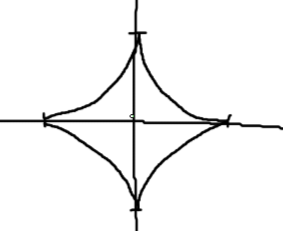
\includegraphics[width=0.4\linewidth]{p5.png}
\end{center}
$\begin{aligned}[t]
	x^{2/3}+y^{2/3}=1
	&\implies y^{2/3}=1-x^{2/3}
	\implies y=\left(1-x^{2/3}\right)^{3/2} \\
	&\implies \frac23 x^{-1/3}+\frac23 y^{-1/3}\cdot\diff yx=0
	\implies y^{-1/3}\cdot\diff yx=-x^{-1/3}
	\implies \frac{1}{\sqrt[3]{y}}\diff yx=-\frac{1}{\sqrt[3]{x}} \\
	&\implies \diff yx=-\frac{\sqrt[3]{y}}{\sqrt[3]{x}}
	=-\frac{\sqrt[3]{\left(1-x^{2/3}\right)^{3/2}}}{\sqrt[3]{x}}
	=-\frac{\left(1-x^{2/3}\right)^{1/2}}{\sqrt[3]{x}}
	=-\frac{\sqrt{1-x^{2/3}}}{\sqrt[3]{x}}
\end{aligned}$

$\begin{aligned}[t]
	L&=4 \int_{0}^{1}\sqrt{1+\left(\diff yx\right)^2}\,\mathrm{d}x
	 =4 \int_{0}^{1}\sqrt{1+\left(-\frac{\sqrt{1-x^{2/3}}}{\sqrt[3]{x}}\right)^2}\,\mathrm{d}x
	 =4 \int_{0}^{1}\sqrt{\frac{\left(\sqrt[3]{x}\right)^2}{\left(\sqrt[3]{x}\right)^2}+\frac{1- \left(\sqrt[3]{x}\right)^2}{\left(\sqrt[3]{x}\right)^2}}\,\mathrm{d}x \\
	 &=4 \int_{0}^{1}\sqrt{\frac{1}{\left(\sqrt[3]{x}\right)^2}}\,\mathrm{d}x
	 =4 \int_{0}^{1}\frac{1}{\sqrt[3]{x}}\,\mathrm{d}x
	 =4 \int_{0}^{1}x^{-1/3}\,\mathrm{d}x
	 =4 \left[\frac{x^{2/3}}{2/3}\right]_{0}^{1}
	 =4\cdot\frac32 \left(1-0\right)
	 =\boxed{6}
\end{aligned}$

\problem{6}
$\begin{aligned}[t]
	&180-\frac{x^2}{45}=0
	\implies \frac{x^2}{45}=180
	\implies x^2=8100
	\implies x=\pm90
	\implies x=90
\end{aligned}$
(keep only positive root)
\newline

$\begin{aligned}[t]
	D&=\int_{0}^{90}\sqrt{1+\left(\deriv[x]\left[180-\frac{x^2}{45}\right]\right)^2}\,\mathrm{d}x
	=\int_{0}^{90}\sqrt{1+\left(-\frac{2x}{45}\right)^2}\,\mathrm{d}x
	=\int_{0}^{90}\sqrt{1+\frac{4x^2}{45^2}}\,\mathrm{d}x
	\approx \boxed{209.1\si{\meter}}
\end{aligned}$

\problem{7}
$\begin{aligned}[t]
	L&=\int_{1}^{4}\sqrt{1+\left(\diff yx\right)^2}\,\mathrm{d}x
	=\int_{1}^{4}\sqrt{1+\left(\deriv[x]\int_{1}^{x}\sqrt{t^3-1}\,\mathrm{d}t\right)^2}\,\mathrm{d}x
	=\int_{1}^{4}\sqrt{1+\big(\sqrt{x^3-1}\big)^2}\,\mathrm{d}x \\
	&=\int_{1}^{4}\sqrt{1+x^3-1}\,\mathrm{d}x
	=\int_{1}^{4}x^{3/2}\,\mathrm{d}x
	=\left[\frac{x^{5/2}}{5/2}\right]_{1}^{4}
	=\frac25 \left(32-1\right)
	=\frac{2\cdot31}{5}
	=\boxed{\frac{62}{5}}
\end{aligned}$

\end{document}
